\documentclass[11pt]{article}
\usepackage[T1]{fontenc}
\usepackage[utf8]{inputenc}
\usepackage{enumerate}
\usepackage{setspace}
\usepackage{amsmath,amssymb,amsthm}
\usepackage{graphicx}
\usepackage{bbm}
\usepackage[round]{natbib}
\usepackage[nohead]{geometry}
\usepackage[bottom]{footmisc}
\usepackage{indentfirst}
\usepackage{endnotes}
\usepackage{graphicx}%
\usepackage{eurosym}
\usepackage{array}
\usepackage{siunitx}
\usepackage{booktabs}
\usepackage{tabularx}
\usepackage[flushleft]{threeparttable}
\usepackage{caption}
\usepackage{subcaption}
\usepackage{rotating}
% \usepackage[hidelinks]{hyperref}
\usepackage{floatrow} %[capposition=top]
\floatsetup{footposition=bottom,capposition=top}
\renewcommand{\labelitemi}{--}
\renewcommand{\labelitemii}{$\bullet$}
\bibliographystyle{chicago}
% \geometry{left=1in,right=1in,top=1.00in,bottom=1.0in}
\let\olditemize\itemize
\renewcommand{\itemize}{
  \olditemize
  \setlength{\itemsep}{-1pt}
}

\begin{document}

\title{Physician fees and densities in Paris%
\thanks{Data available upon request, all comments are welcome.%
}}

\author{Etienne Chamayou\thanks{e-mail:
\textit{etienne.chamayou@ensae.fr}}\medskip\\{\normalsize CREST and Department of Economics, Ecole Polytechnique }}
\maketitle

\sloppy%

\onehalfspacing

\textbf{Abstract:}

This note compares the fees and densities of general practitioners and ophthalmologists in Paris. A large majority of ophthalmologists can freely chose their price policy (sector 2), while most general practitioners follow fee policies determined by law (sector 1). Using data from the French National Health Service, this note shows that the density and prices of sector 2 physicians, irrespective of their specialty, are strongly correlated to revenue at the Paris arrondissement level. Since most ophthalmologists are sector 2, the densities of ophthalmologists across arrondissements exhibit large inequalities, while general practitioners are more evenly geographically distributed. The 5\textsuperscript{th} highest income district has a 180\% higher opthalmologist density, respectively 50\% higher general practitioner density, than the 5\textsuperscript{th} lowest income district.

\strut

\pagebreak%
\doublespacing

\section{Introduction}

Local physician shortages are a growing health policy issue in France. Among the various specialties, ophthalmology is one of the most affected. It is also characterized by a high proportion of sector 2 practitioners, who are not subject to regulated fees. Conversely, most general practitioners belong to sector 1 and thus perceive fees determined by law. While the debate about healthcare regulation certainly belongs in the public sphere, the scarcity of information makes it difficult to develop an informed opinion. A most controversial issue is the extent to which healthcare is or should be a market.

This note compares the fees and densities of general practitioners and ophthalmologists in Paris. Prices of general practitioners are largely regulated, hence the only way to increase income for most of them is to increase the number of consultations. Conversely, many ophthalmologists freely chose their price policy. They can thus increase revenue through higher fees, which gives them an incentive to settle in wealthier areas.

Using data from the French National Health Service, this note shows that the densities and fees of sector 2 physicians, irrespective of their specialty, are strongly correlated to revenue at the Paris arrondissement level. Since most ophthalmologists are sector 2, the densities of ophthalmologists across arrondissements exhibit large inequalities, while general practitioners are more evenly distributed. The 5\textsuperscript{th} highest income district has a 180\% higher opthalmologist density, respectively 50\% higher general practitioner density, than the 5\textsuperscript{th} lowest income district.

\section{Data}

Physician locations and fees were collected in 2014 from the website annuairesante.ameli.fr, a website operated by the French National Health Service meant to foster access to healthcare. The website includes all active physicians except for pure hospital practitioners. Data were aggregated at the "arrondissement" level in Paris, and matched with socio-demographic data from the French 2010 national census and fiscal data. The variable used to account for population revenue by arrondissement is the median fiscal revenue by consumption unit (Household declared revenues are weighted according to OECD methodology). The share of people aged over 65 in the arrondissement is used to account for variations in demand related to ageing. The analysis focuses on basic consultation fees. Regarding sector 1 physicians, they amount to 23 euros for general practitioners, and 28 euros for ophthalmologists at the time of the study. In sector 2, the average fees in Paris are respectively 38 and 65 euros. Descriptive statistics are provided in Tables~\ref{tab:GP_stats_des} and \ref{tab:Ophthalmo_stats_des}. Data contain 2,488 general practitioners, of which 58\% belong to sector 1, 35\% belong to sector 2 and 7\% to neither of them. Similarly, there are 450 listed ophthalmologists, of which 15\% belong to sector 1 and 85\% to sector 2. All physician densities are expressed per 100,000 inhabitants.

\section{General Practitioners}

The overall densities of GPs are bunched around 100 and 150, and appear to be moderately correlated with income (cf. Figure~\ref{fig:GP_densities}). The 8th district constitute an outlier given its unusually high physician density, above 300. A correlation with revenue can be most clearly observed for the density of sector 2 GPs i.e. physicans who choose their price policy (cf. Figure~\ref{fig:GP_s2_densities}). The same pattern can be observed with the average consultation fees (cf. Figure~\ref{fig:GP_s2_fees}). Results of regressions of sector 2 GP densities and fees on revenue and share of people aged over 65 are provided in Table~\ref{tab:regs_density_fees}.

\begin{figure}[H]
    \caption{Density of GPs vs. revenue by district}
		\label{fig:GP_densities}
	\centering
		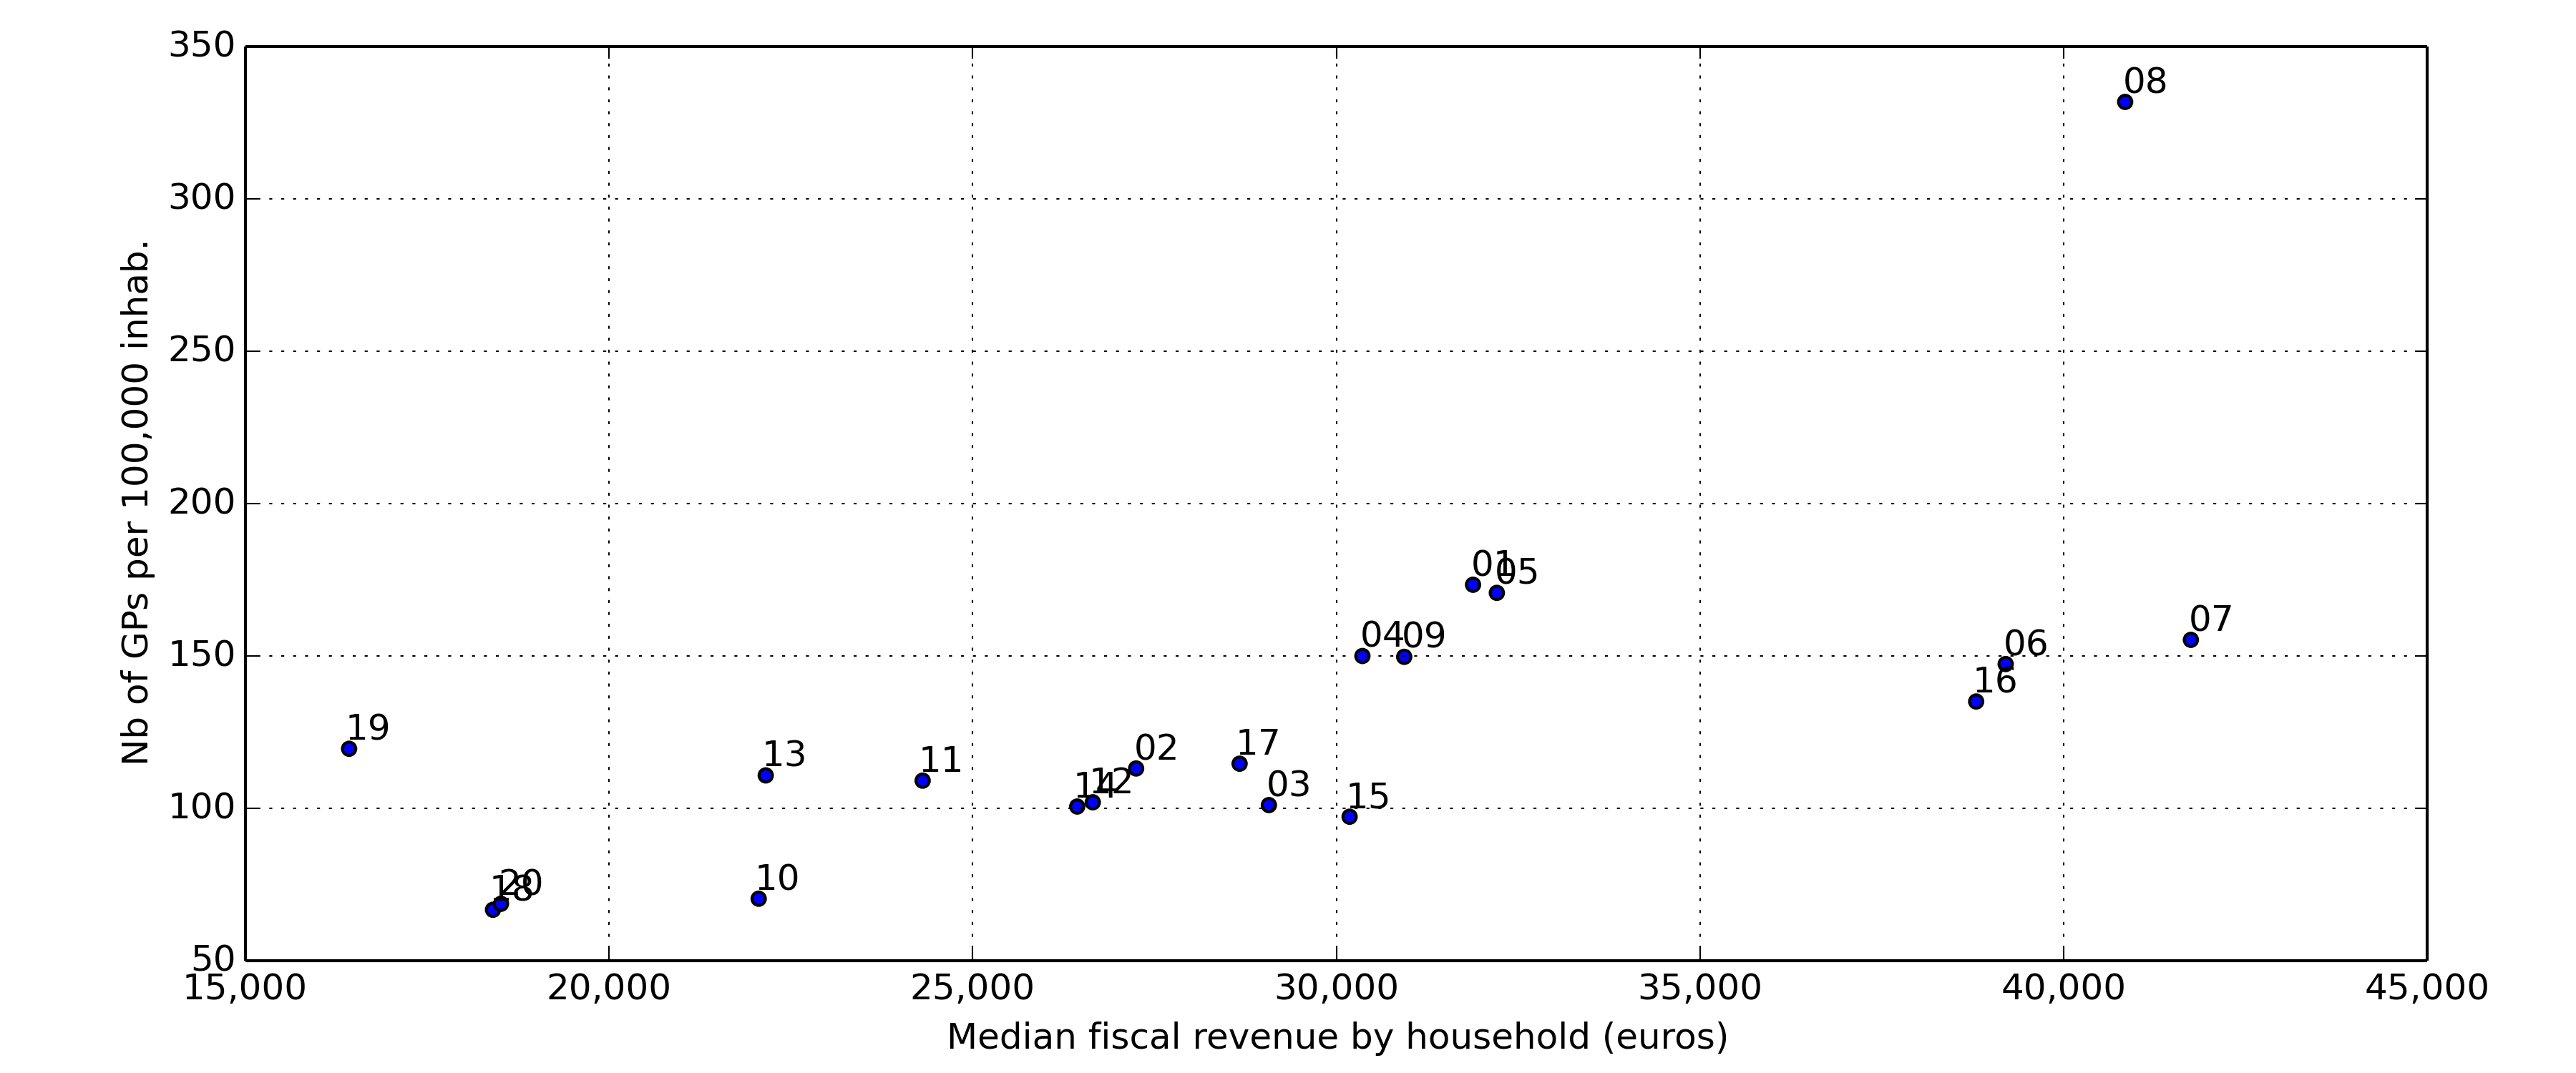
\includegraphics[width=16cm]{images/GP_Ardt_DensityVsRevenue.png}
\end{figure}

\begin{figure}[H]
    \caption{Density of sector 1 GPs vs. revenue by district}
		\label{fig:GP_s1_densities}
	\centering
		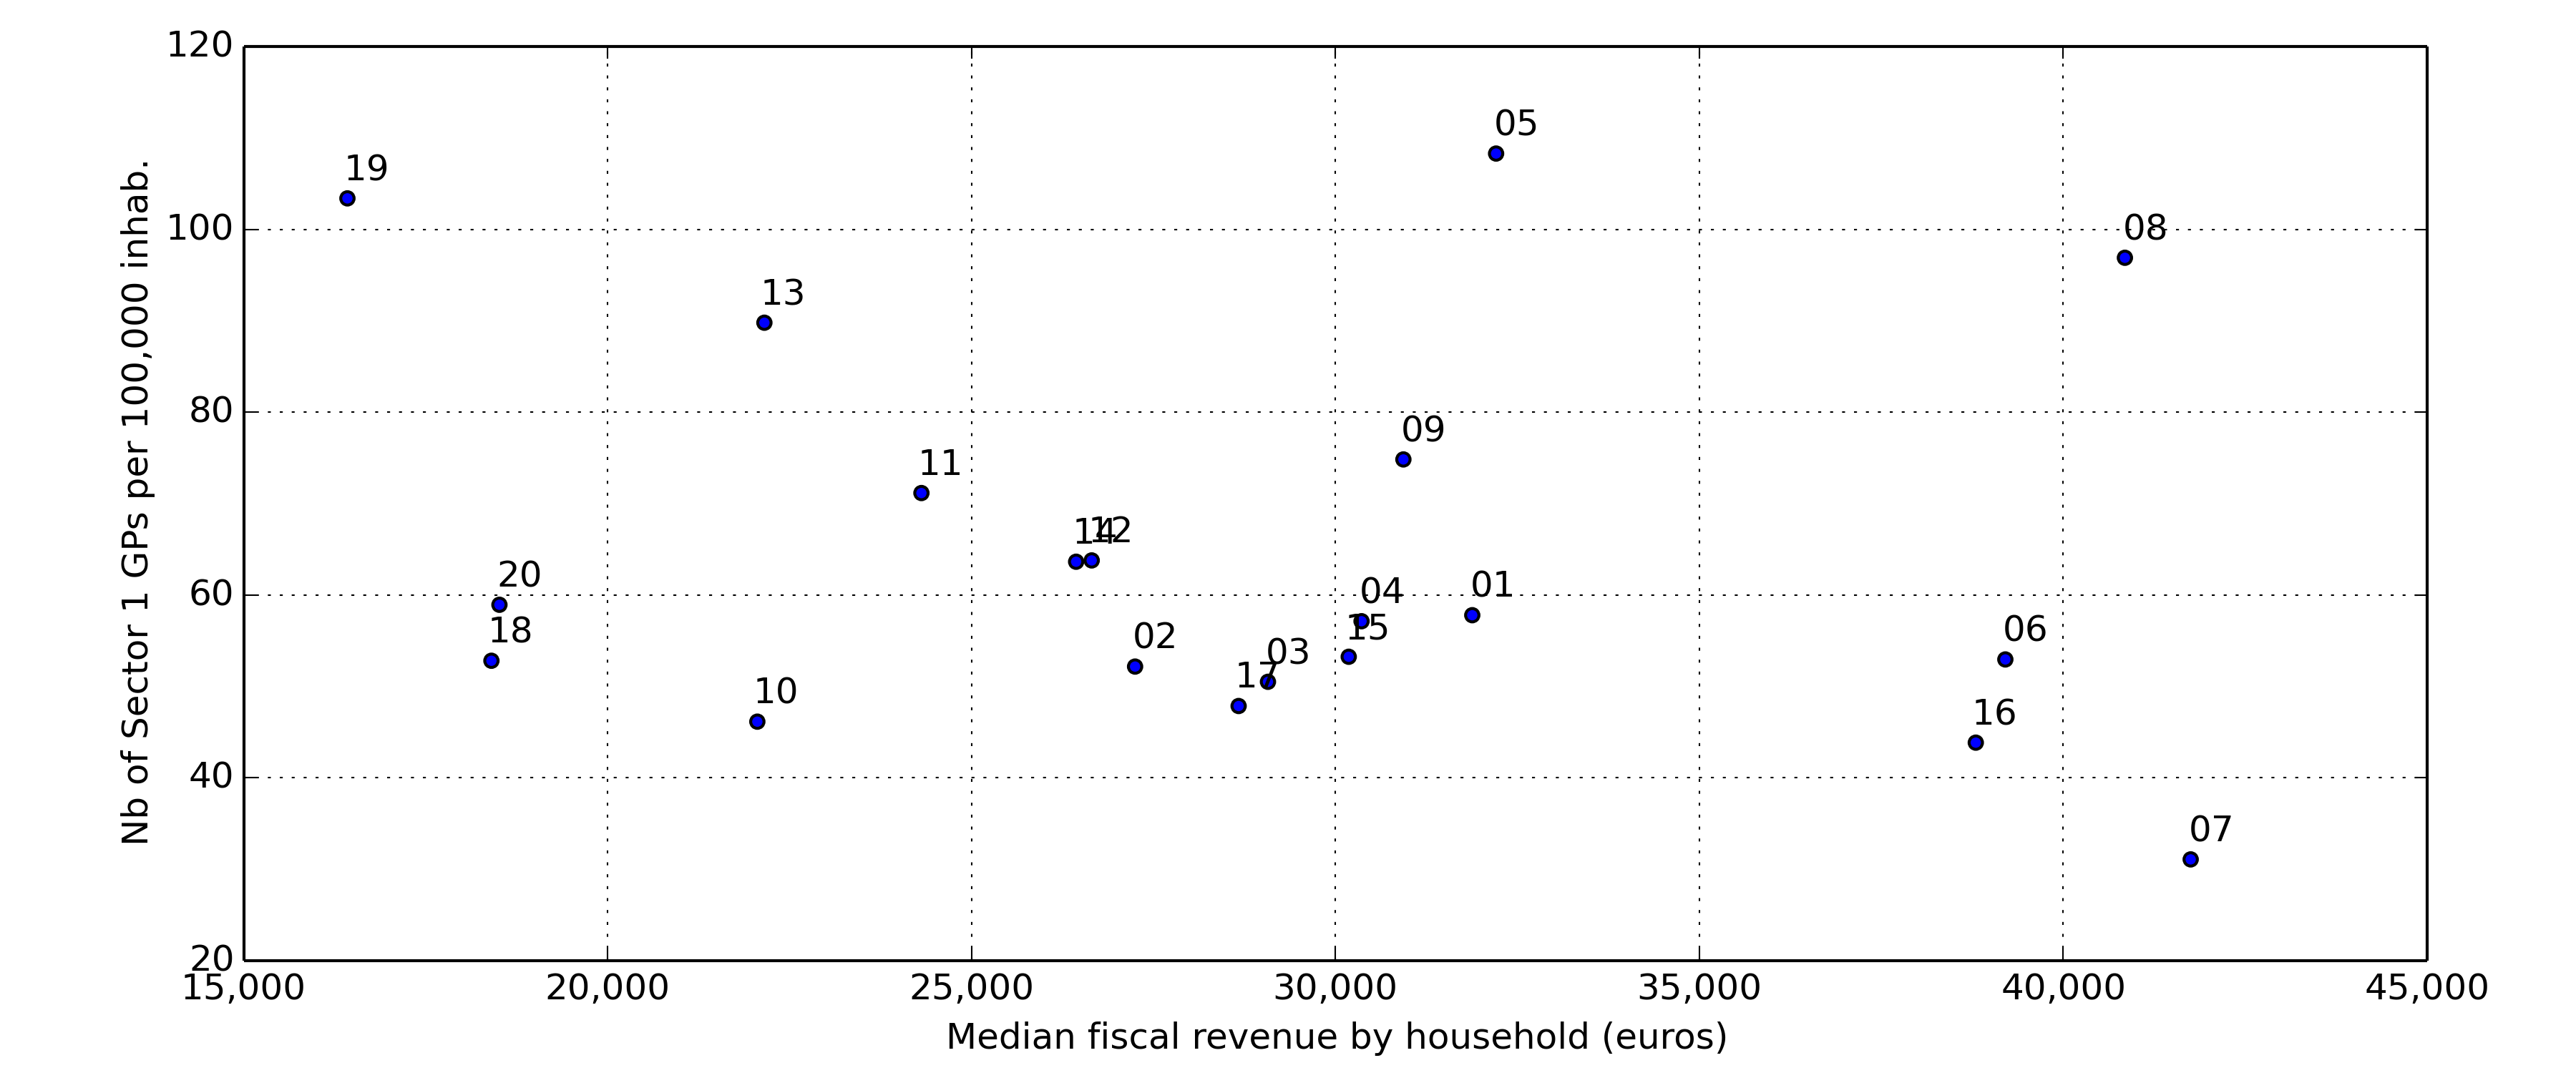
\includegraphics[width=16cm]{images/GP_Ardt_DensityS1VsRevenue.png}
\end{figure}

\begin{figure}[H]
    \caption{Density of sector 2 GPs vs. revenue by district}
		\label{fig:GP_s2_densities}
	\centering
		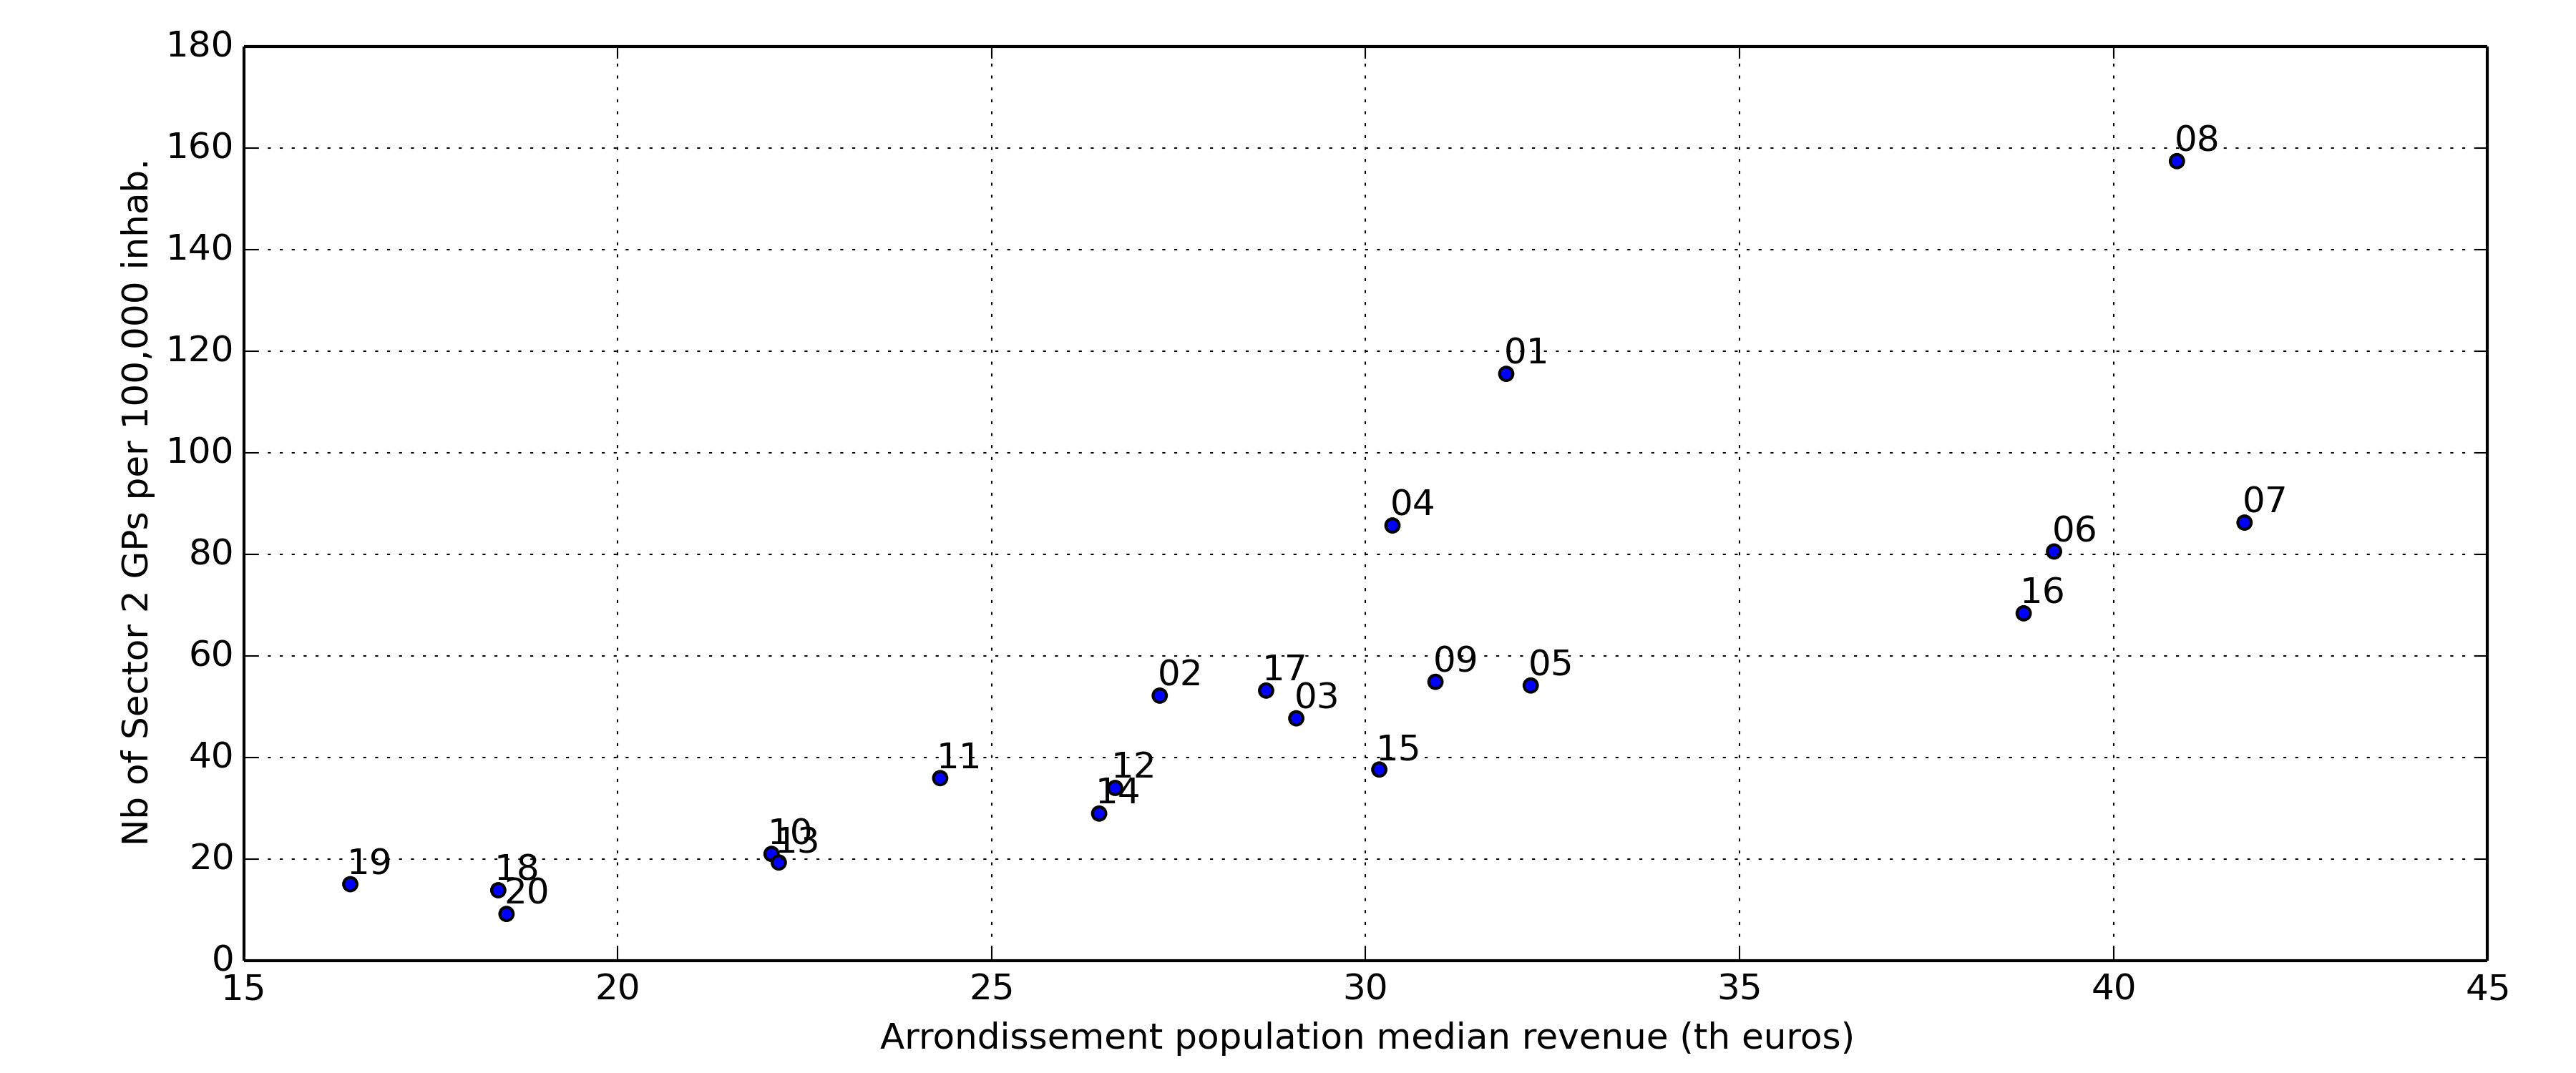
\includegraphics[width=16cm]{images/GP_Ardt_DensityS2VsRevenue.png}
\end{figure}

\begin{figure}[H]
    \caption{Sector 2 GP consultation fees vs. revenue by district}
		\label{fig:GP_s2_fees}
	\centering
		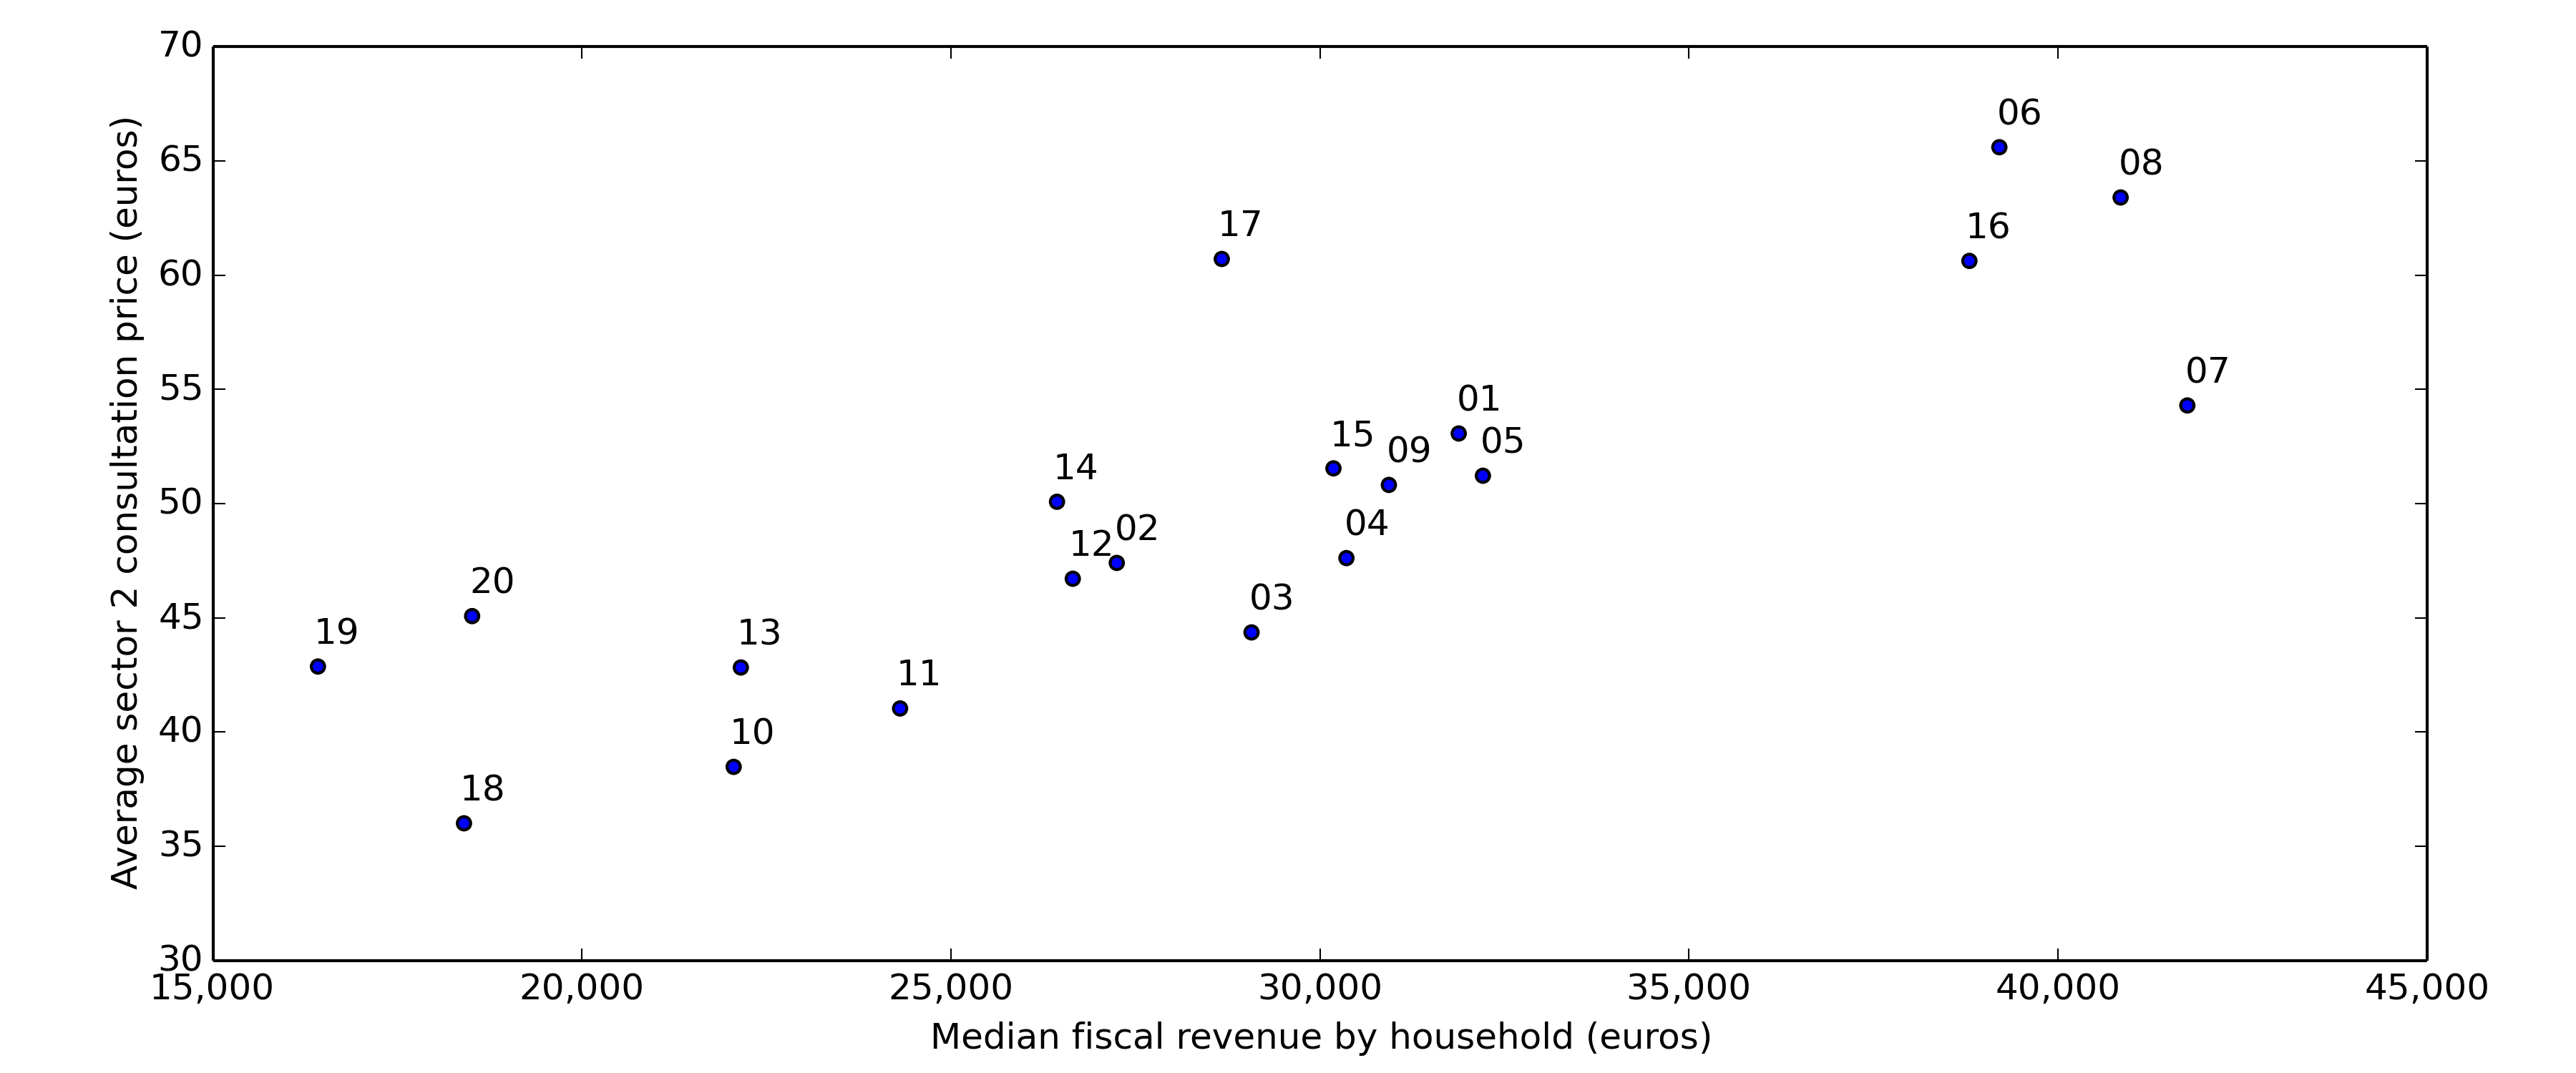
\includegraphics[width=16cm]{images/GP_Ardt_ConsultationS2VsRevenue.png}
\end{figure}

\section{Ophthalmologists}

The number of ophthalmologists per inhabitant exhibits stronger correlation with revenue than in the case of GPs (cf. Figure~\ref{fig:Ophtalmo_s2_fees}). The density of sector 1 ophthalmologists is relatively stable across districts, but these account for a small portion of ophthalmologists in Paris. Both the density of sector 2 ophthalmologists and their average consultation price are largely correlated with revenue (cf. Figure~\ref{fig:Ophtalmo_s2_densities} and \ref{fig:Ophtalmo_s2_fees}). Results of regressions of sector 2 ophthalmologists densities and fees on revenue and share of people aged over 65 are provided in Table~\ref{tab:regs_density_fees}.

\begin{figure}[H]
    \caption{Density ophtalmologists vs. revenue by district}
		\label{fig:Ophtalmo_densities}
	\centering
		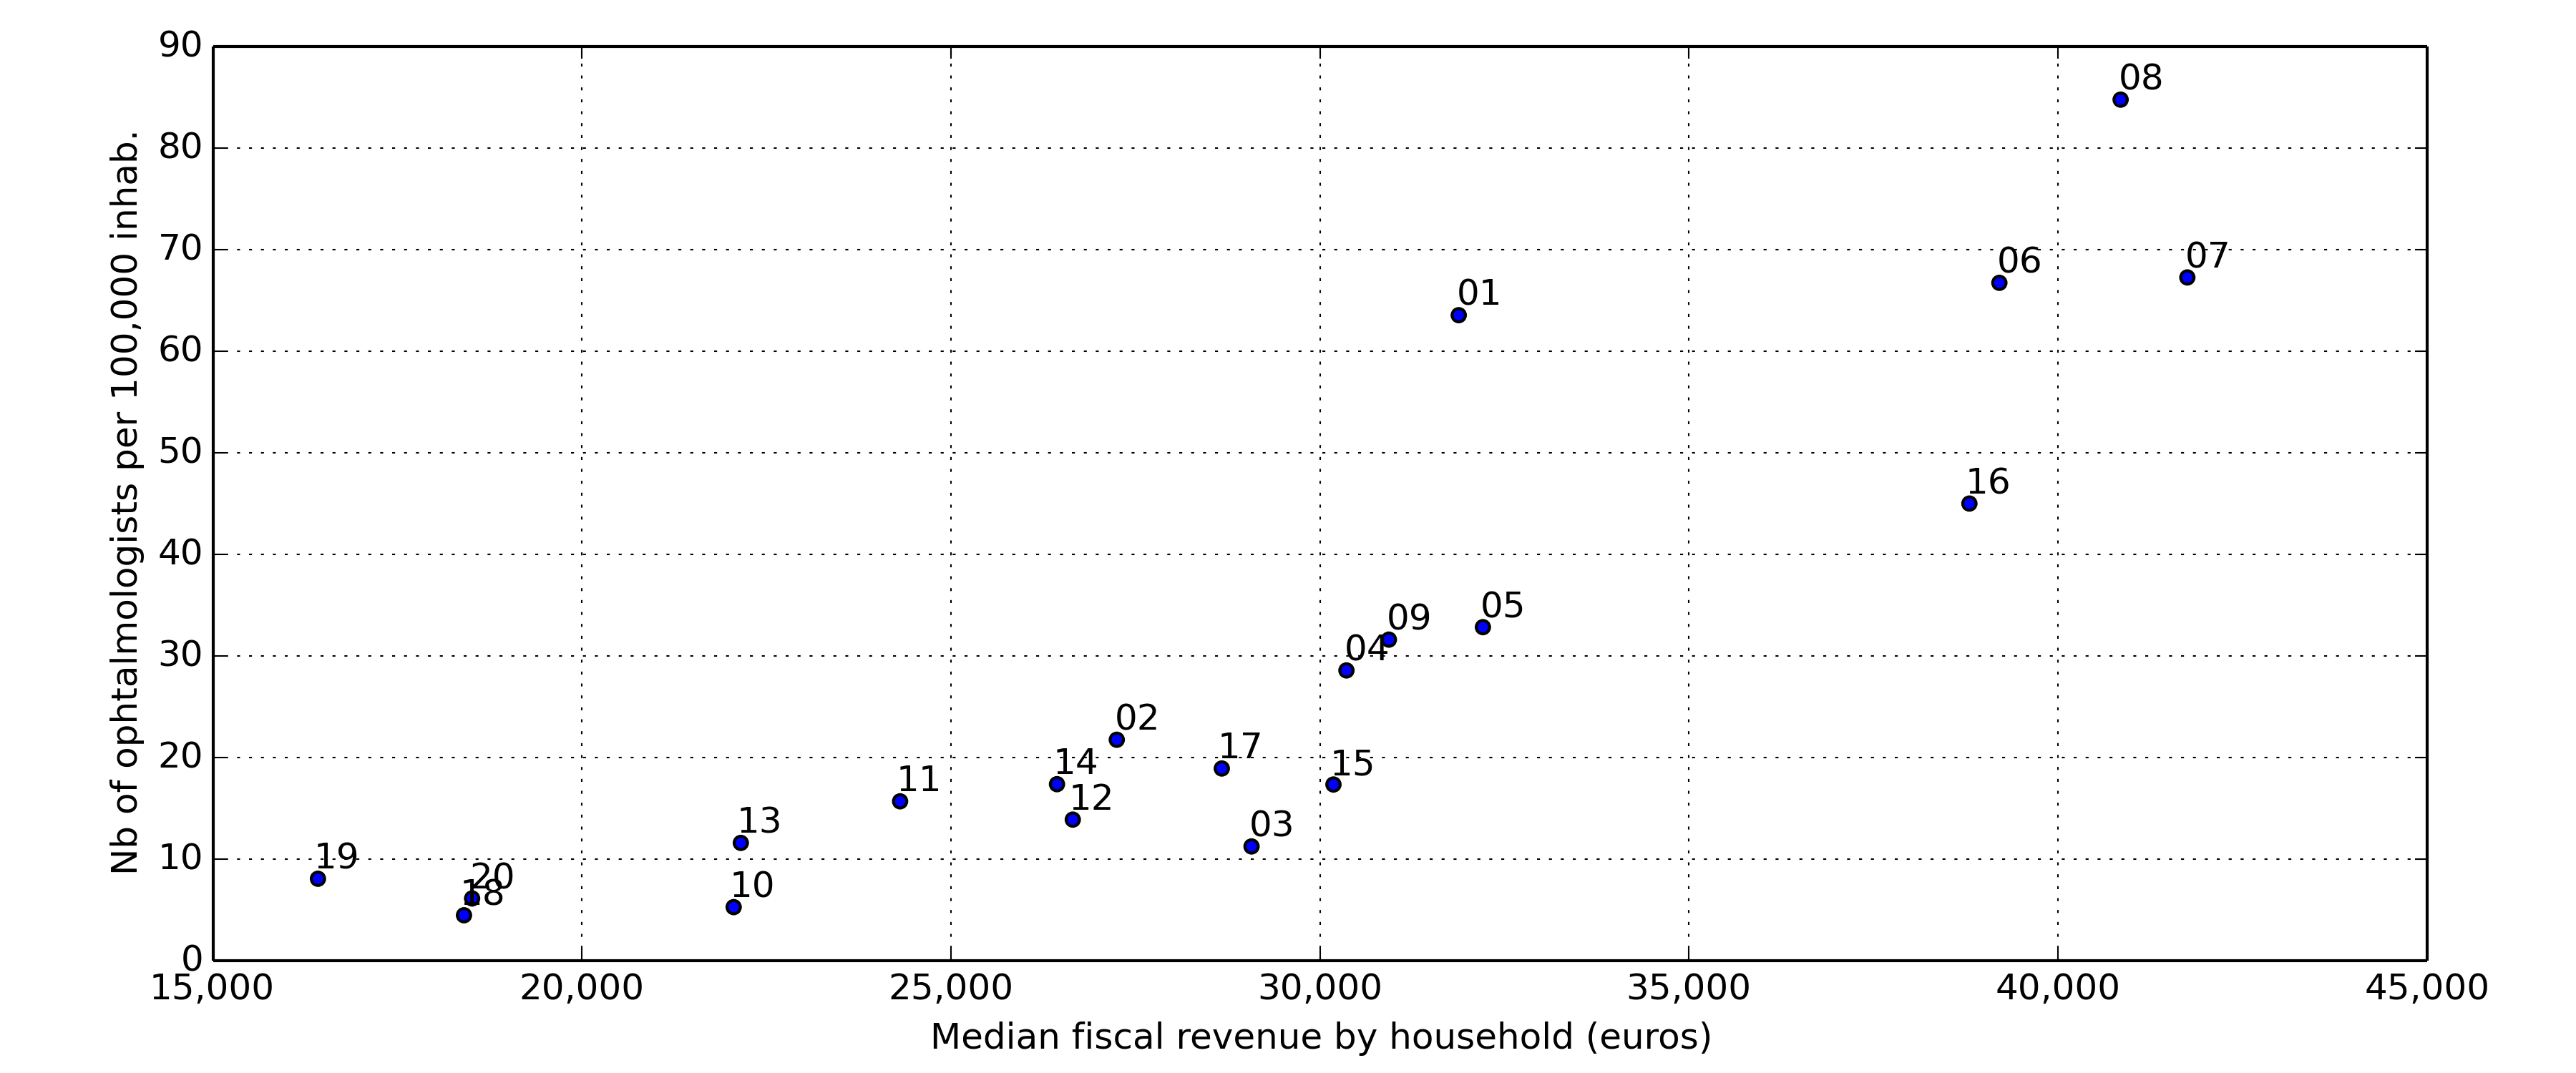
\includegraphics[width=16cm]{images/Ophtalmo_Ardt_DensityVsRevenue.png}
\end{figure}

\begin{figure}[H]
    \caption{Density of sector 1 ophtalmologists vs. revenue by district}
		\label{fig:Ophtalmo_s1_densities}
	\centering
		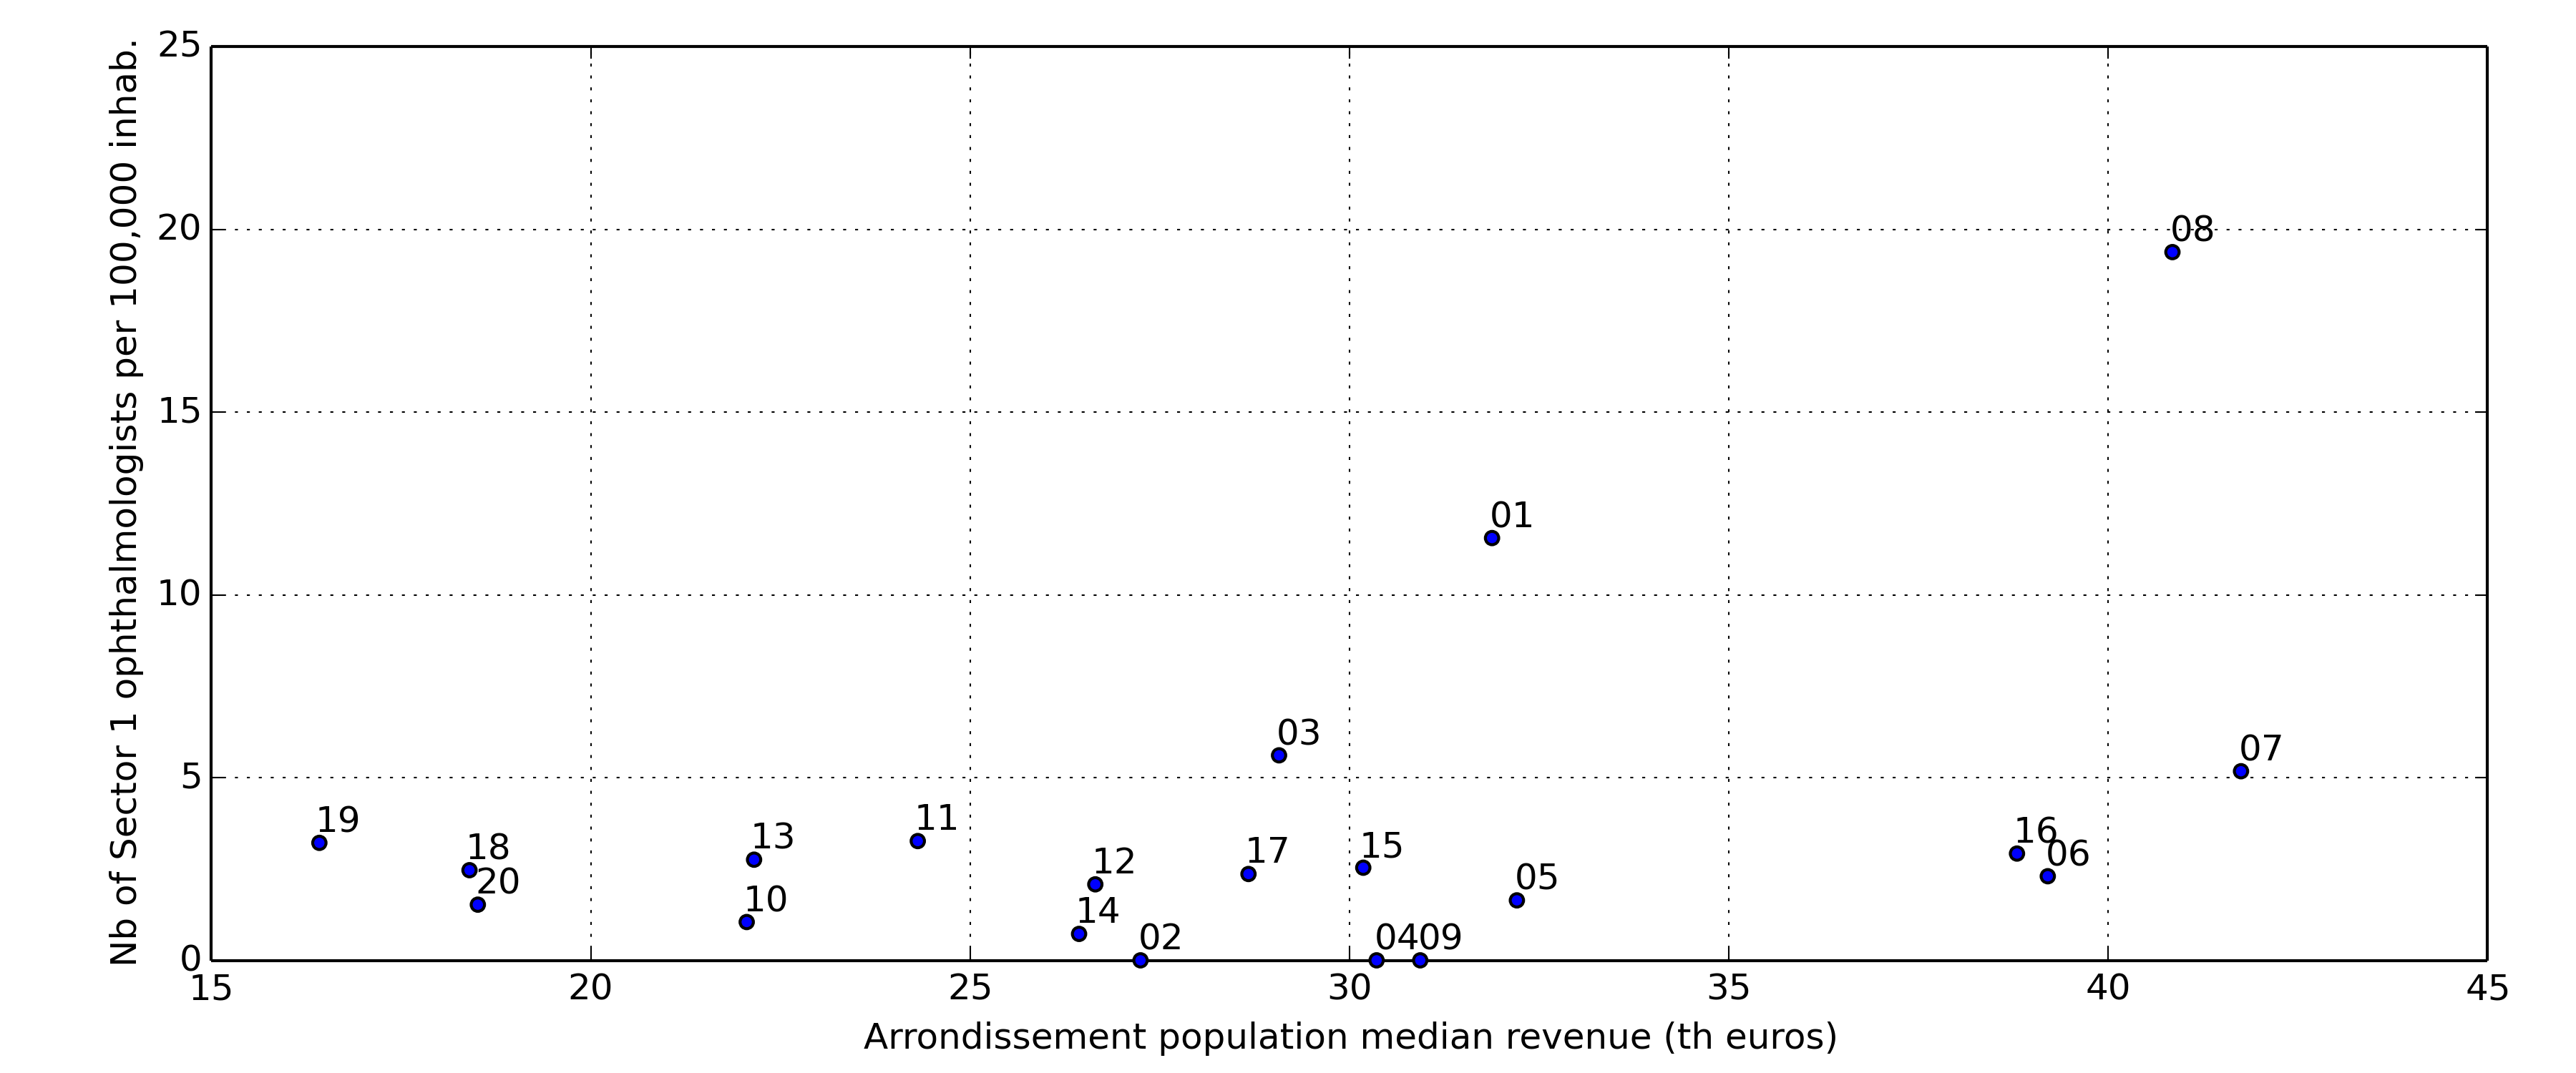
\includegraphics[width=16cm]{images/Ophtalmo_Ardt_DensityS1VsRevenue.png}
\end{figure}


\begin{figure}[H]
    \caption{Density of sector 2 ophtalmologists vs. revenue by district}
		\label{fig:Ophtalmo_s2_densities}
	\centering
		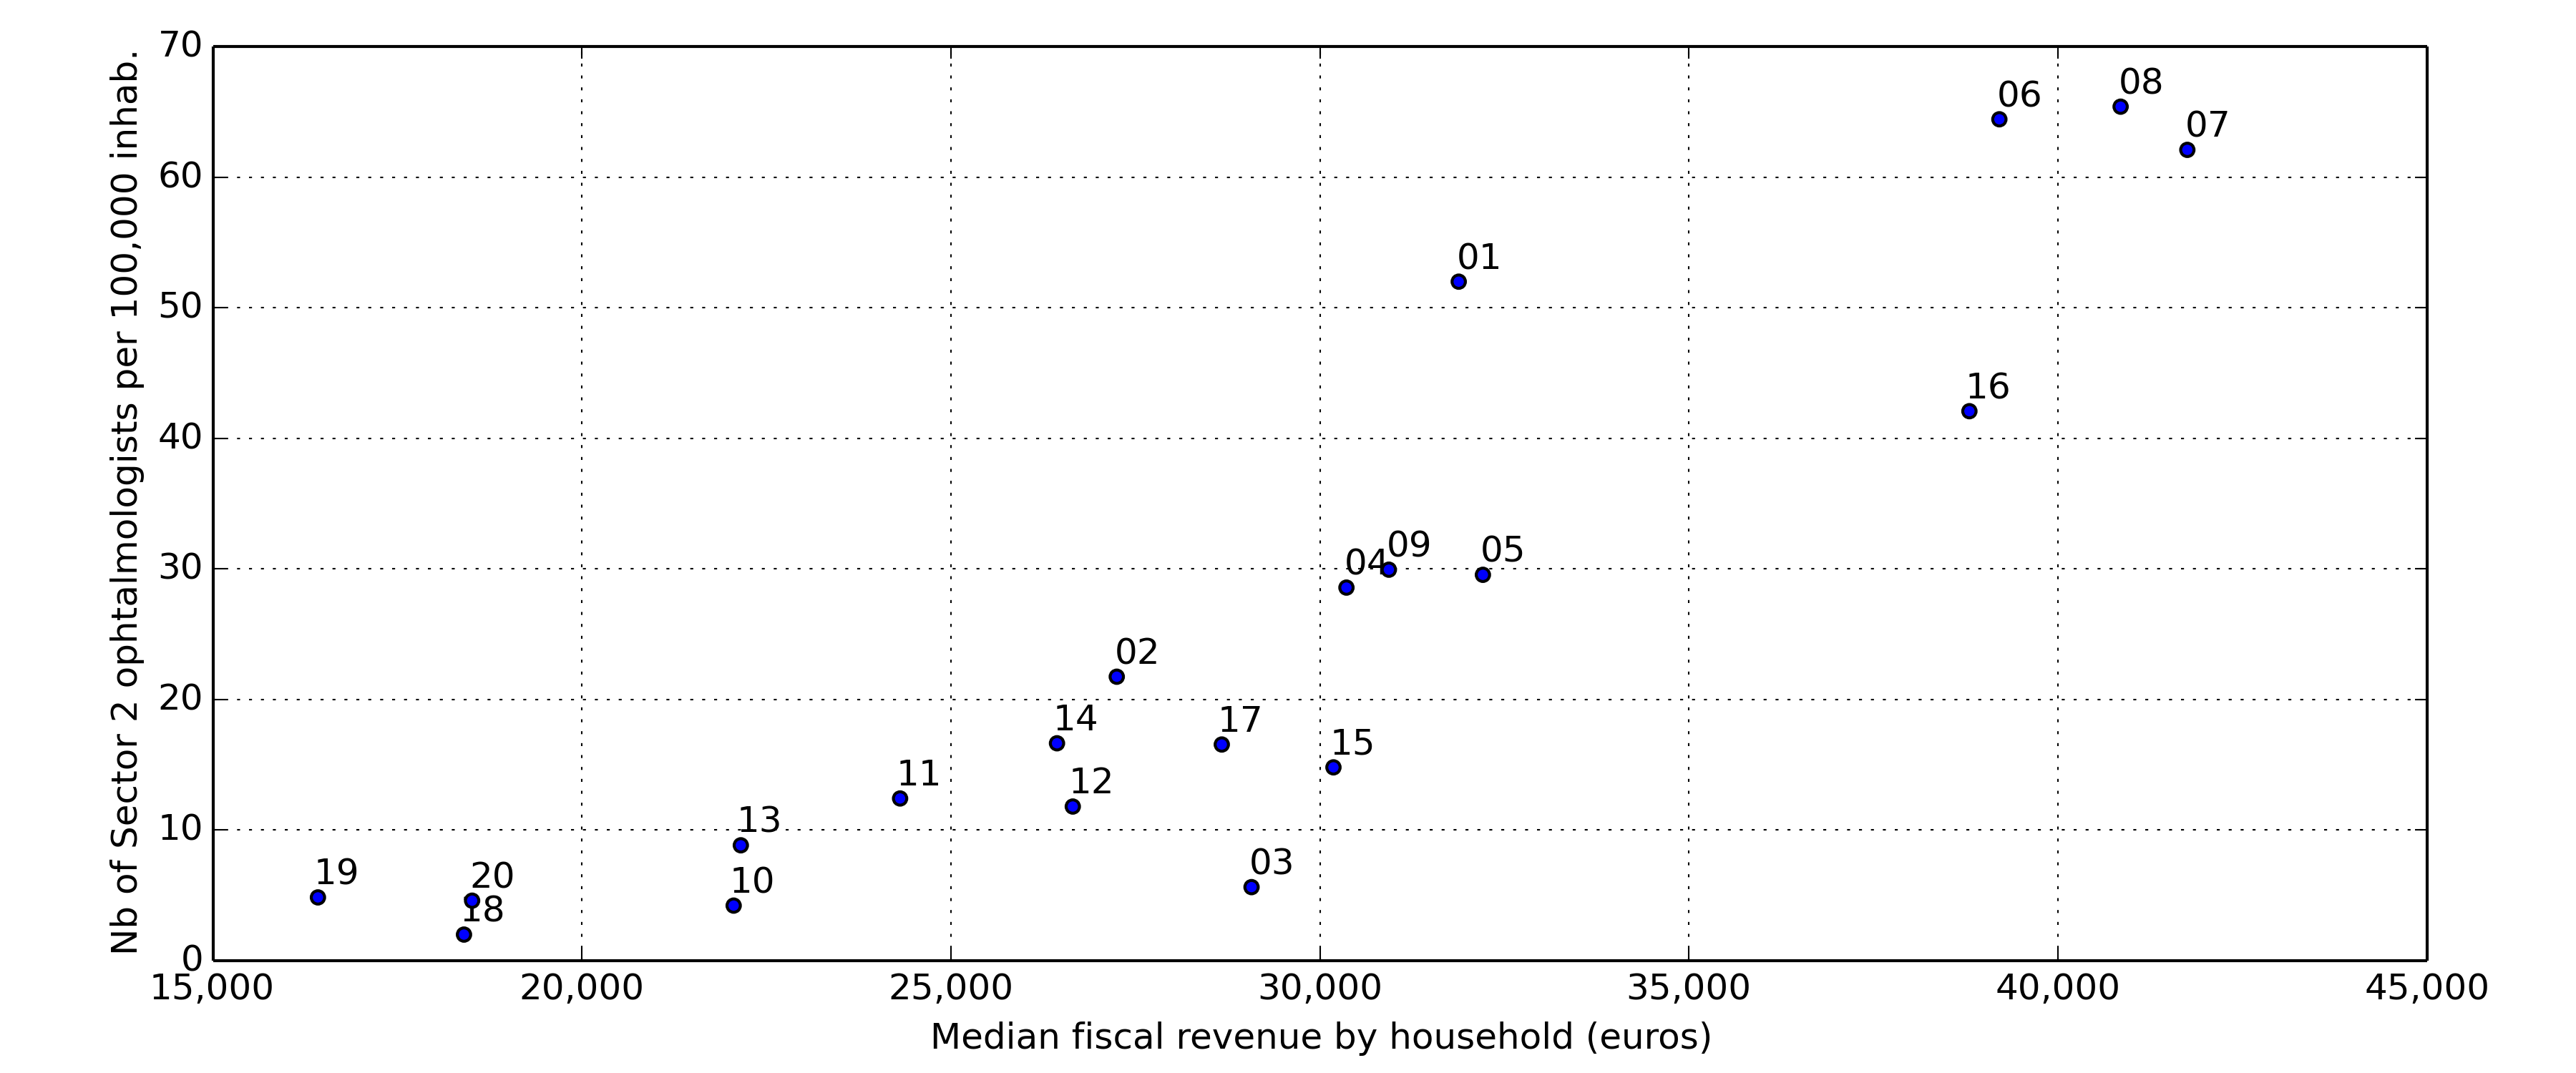
\includegraphics[width=16cm]{images/Ophtalmo_Ardt_DensityS2VsRevenue.png}
\end{figure}

\begin{figure}[H]
    \caption{Sector 2 ophtalmologist fees vs. revenue by district}
		\label{fig:Ophtalmo_s2_fees}
	\centering
		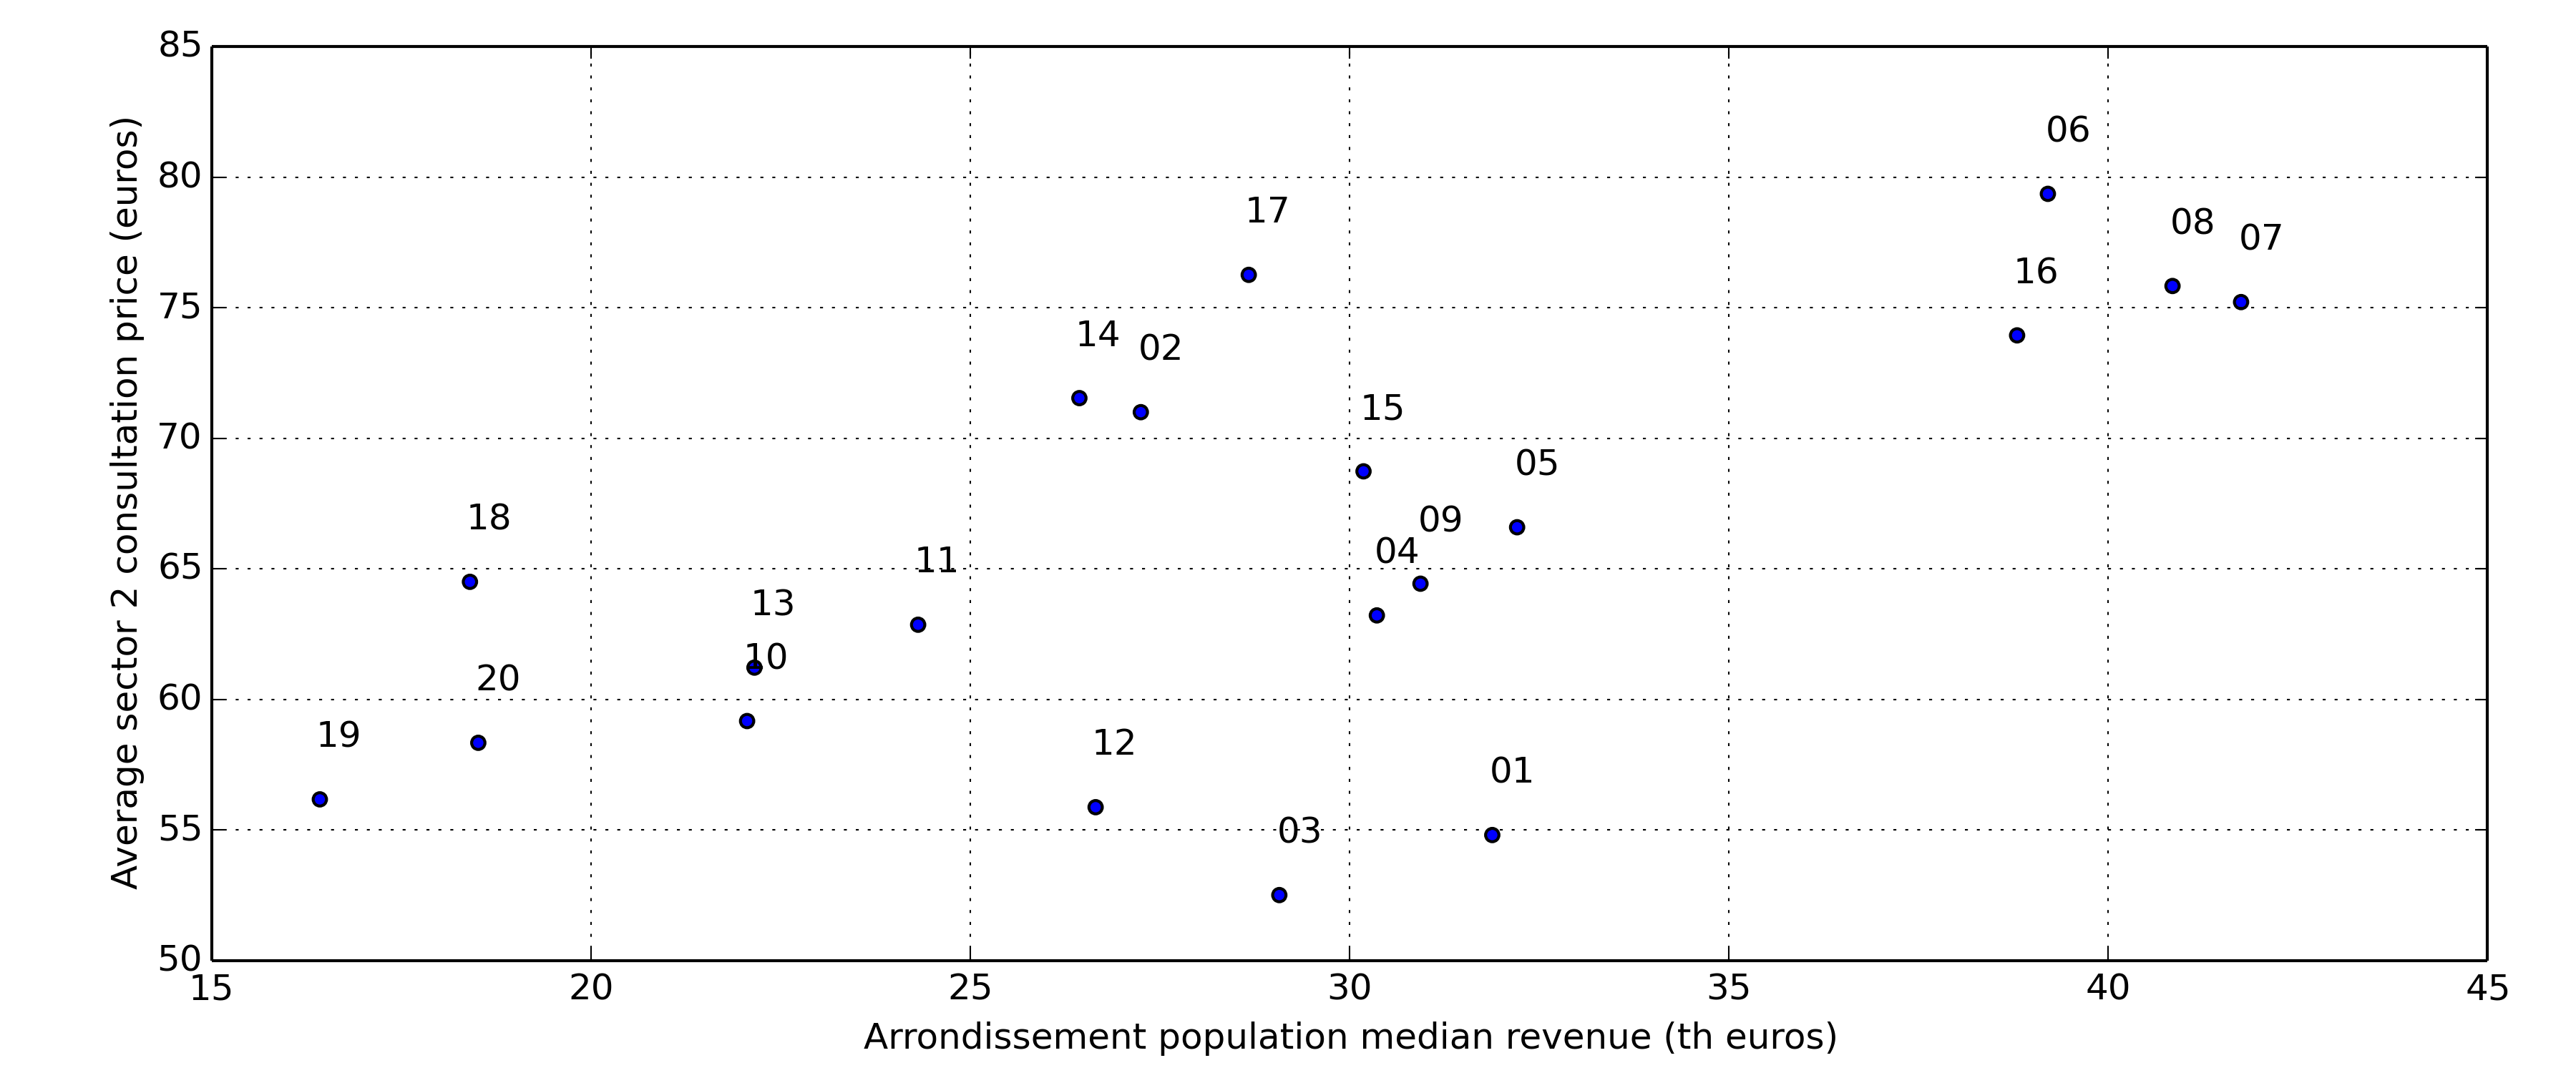
\includegraphics[width=16cm]{images/Ophtalmo_Ardt_ConsultationS2VsRevenue.png}
\end{figure}

\clearpage

\appendix

\section{Descriptive statistics}

\begin{table}[h]
\caption{Overview of general practitioners by arrondissement}
\label{tab:GP_stats_des}
\begin{tabular}{lrrrrrrr}
\hline
\hline
Arrondis-      & Pop.      & Aged       & Med. rev.  & Phys.  & Sec. 2  & Sec. 2 fee  & Sec. 2 fee  \\
sement         & (th)      & 65+ (\%)   & (th euros) & sity   & density & avg (euros) & std (euros) \\
\hline
1     & 17    & 19    & 32    & 173   & 116   & 53    & 16 \\
2     & 23    & 14    & 27    & 113   & 52    & 47    & 10 \\
3     & 36    & 18    & 29    & 101   & 48    & 44    & 17 \\
4     & 28    & 22    & 30    & 150   & 86    & 48    & 17 \\
5     & 61    & 23    & 32    & 171   & 54    & 51    & 21 \\
6     & 43    & 27    & 39    & 147   & 81    & 66    & 25 \\
7     & 58    & 27    & 42    & 155   & 86    & 54    & 17 \\
8     & 41    & 21    & 41    & 332   & 157   & 63    & 21 \\
9     & 60    & 16    & 31    & 150   & 55    & 51    & 18 \\
10    & 95    & 14    & 22    & 70    & 21    & 38    & 20 \\
11    & 153   & 18    & 24    & 109   & 36    & 41    & 16 \\
12    & 144   & 21    & 27    & 102   & 34    & 47    & 15 \\
13    & 182   & 21    & 22    & 111   & 19    & 43    & 15 \\
14    & 138   & 21    & 26    & 101   & 29    & 50    & 20 \\
15    & 237   & 21    & 30    & 97    & 38    & 52    & 18 \\
16    & 171   & 27    & 39    & 135   & 68    & 61    & 20 \\
17    & 169   & 20    & 29    & 115   & 53    & 61    & 22 \\
18    & 203   & 17    & 18    & 67    & 14    & 36    & 12 \\
19    & 187   & 17    & 16    & 119   & 15    & 43    & 17 \\
20    & 197   & 18    & 19    & 69    & 9     & 45    & 21 \\
\hline
Tot. & 2,244  & 20    & 25    & 111   & 38    & 52    & 20 \\
\hline
\hline
\end{tabular}%
\end{table}

\begin{table}[h]
\caption{Overview of ophthalmologists by arrondissement}
\label{tab:Ophthalmo_stats_des}
\begin{tabular}{lrrrrrrr}
\hline
\hline
Arrondis-      & Pop.      & Aged       & Med. rev.  & Phys.  & Sec. 2  & Sec. 2 fee  & Sec. 2 fee  \\
sement         & (th)      & 65+ (\%)   & (th euros) & sity   & density & avg (euros) & std (euros) \\
\hline
1     & 17    & 19    & 32    & 64    & 52    & 55    & 30 \\
2     & 23    & 14    & 27    & 22    & 22    & 71    & 17 \\
3     & 36    & 18    & 29    & 11    & 6     & 52    & 18 \\
4     & 28    & 22    & 30    & 29    & 29    & 63    & 8 \\
5     & 61    & 23    & 32    & 30    & 30    & 67    & 12 \\
6     & 43    & 27    & 39    & 33    & 64    & 79    & 32 \\
7     & 58    & 27    & 42    & 67    & 62    & 75    & 13 \\
8     & 41    & 21    & 41    & 85    & 65    & 76    & 18 \\
9     & 60    & 16    & 31    & 32    & 30    & 64    & 10 \\
10    & 95    & 14    & 22    & 5     & 4     & 59    & 14 \\
11    & 153   & 18    & 24    & 16    & 12    & 63    & 11 \\
12    & 144   & 21    & 27    & 14    & 12    & 56    & 13 \\
13    & 182   & 21    & 22    & 12    & 9     & 61    & 10 \\
14    & 138   & 21    & 26    & 17    & 17    & 72    & 11 \\
15    & 237   & 21    & 30    & 17    & 15    & 69    & 20 \\
16    & 171   & 27    & 39    & 45    & 42    & 74    & 18 \\
17    & 169   & 20    & 29    & 19    & 17    & 76    & 15 \\
18    & 203   & 17    & 18    & 4     & 2     & 64    & 3 \\
19    & 187   & 17    & 16    & 8     & 5     & 56    & 9 \\
20    & 197   & 18    & 19    & 6     & 5     & 58    & 6 \\
\hline
Tot. & 2,244  & 20    & 25    & 19    & 17    & 69    & 18 \\
\hline
\hline
\end{tabular}%
\end{table}

\clearpage

\section{Regressions}

\begin{table}[h]
\begin{threeparttable}
\renewcommand{\arraystretch}{0.8} % too large by default...
\caption{Regressions of densities and fees}
\label{tab:regs_density_fees}
\def\sym#1{\ifmmode^{#1}\else\[^{#1}\]\fi}
\sisetup{table-space-text-post = \sym{***}}
\begin{tabular}{lr*{4}{S[table-align-text-post=false]}} 
\hline
\hline
               & \multicolumn{2}{c}{Sector 2 Density} & \multicolumn{2}{c}{Sector 2 Fee} \\
               & {GP}   & {Ophtalmo} & {GP}   & {Ophtalmo} \\
\hline
{Constant}     & -33.19 & -44.66 & 19.56 & 43.38 \\
				       & [1.33]\sym{} & [3.47]\sym{**} & [3.44]\sym{**} & [5.07]\sym{**} \\
{Pop 65+ (\%)} & -3.43 & 0.42  & 0.38  & 0.10 \\
               & [1.98]\sym{} & [0.51]\sym{} & [0.97]\sym{} & [0.18]\sym{} \\
{Med. revenue} & 5.40  & 2.75  & 0.78  & 0.72 \\
               & [6.01]\sym{**} & [6.51]\sym{**} & [3.80]\sym{**} & [2.55]\sym{*} \\
\hline
{Adj. R2}      & 0.70  & 0.81  & 0.68  & 0.41 \\
{Nb. obs.}     & {20}    & {17}    & {20}    & {17} \\
\hline
\hline
\end{tabular}
\begin{tablenotes}
			\small
			\item T-statistics in square brackets.
      \item {**} p < 1\%, {*} p < 5\%
      \item Arrondissements with less than 5 price observations are dropped hence only 17 are used in the Ophtalmologist regression.
\end{tablenotes}
\end{threeparttable}
\end{table}

\end{document}
